\begin{figure}
  \begin{subfigure}{\textwidth}
    \begin{minipage}{.5\textwidth}
      \centering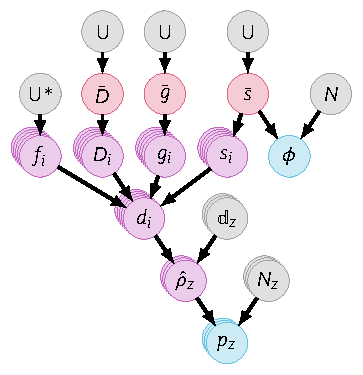
\includegraphics[scale=1]{model.yss}
    \end{minipage}
    \begin{minipage}{.5\textwidth}
      \begin{align}
           p_z &\sim \distr{BAB}{N_z, \hat{\rho}_z} \\
  \hat{\rho}_z &=    \distr{mean}{d_i \in \mathbb{d}_z} \\
           d_i &=    D_i\,(f_i + s_i\,(1 + g_i)) \\
           D_i &\sim \distr{Exp}{1/\bar{D}} \\
           f_i &\sim \distr{Unif}{0,1} \\
           s_i &\sim \distr{Pois}{\bar{s}} \\
           g_i &\sim \distr{Exp}{1/\bar{g}} \\
          \phi &\sim \distr{BAB}{N, 1-e^{-\bar{s}}\,}
      \end{align}
    \end{minipage}
    \caption{Duration selling sex}
    \label{fig:model.yss}
  \end{subfigure}
  \begin{subfigure}{\textwidth}
    \begin{minipage}{.5\textwidth}
      \centering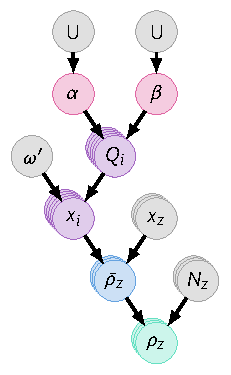
\includegraphics[scale=1]{model.part}
    \end{minipage}
    \begin{minipage}{.5\textwidth}
      \begin{align}
           p_z &\sim \distr{BAB}{N_z, \hat{\rho}_z} \\
  \hat{\rho}_z &=    \distr{mean}{x_i \in \mathbb{x}_z} \\
           x_i &\sim \distr{Pois}{Q_i\,\omega'} \\
           Q_i &\sim \distr{Gamma}{\alpha,\beta}
      \end{align}
    \end{minipage}
    \caption{Rates of partnership change}
    \label{fig:model.part}
  \end{subfigure}
  \caption{Graphical models}
  \label{fig:model}
  \floatfoot{Guide:
    \g{gray}{fixed variable/distribution};
    \g{red}{target};
    \g{purple}{intermediate};
    \g{blue}{observed}.
    Variables:
    % both
    \g{$p_z$}{proportion of population};
    \g{$N_z$}{effective sample size};
    \g{$\hat{\rho}_z$}{empirically estimated $p_z$ mean};
    % yss
    \g{$\mathbb{d}_z$}{range of reported durations selling sex};
    \g{$d_i$}{reported duration at survey};
    \g{$D_i$}{total (eventual) duration};
    \g{$f_i$}{censoring fraction};
    \g{$s_i$}{number of times stopped selling sex};
    \g{$g_i$}{relative gap length};
    \g{$\bar{D}$}{true $D$ mean};
    \g{$\bar{s}$}{true $s$ mean};
    \g{$\bar{g}$}{true $g$ mean};
    \g{$\phi$}{proportion who stopped selling sex at least once};
    % parts
    \g{$\mathbb{x}$}{range of reported partner numbers};
    \g{$x_i$}{reported partner numbers};
    \g{$Q_i$}{partnership change rate};
    \g{$\omega'$}{effective recall period};
    \g{$\alpha,\beta$}{parameters of $Q_i$ distribution}.
    % misc
    Distributions:
    \g{U}{uniform / uninformative};
    \g{BAB}{beta approximation of binomial distribution (see \sref{app.bab})}.
  }
\end{figure}
